\documentclass{anstrans}
%%%%%%%%%%%%%%%%%%%%%%%%%%%%%%%%%%%
\title{Benefits of Siting a Borehole Repository at a Non-operating Nuclear 
Facility}
\author{Jin Whan Bae,$^{*}$ Abraham Lincoln$^{\dagger}$}

\institute{
$^{*}$Dept. of Nuclear Plasma, and Radiological Engineering, University of Illinois at Urbana-Champaign, Urbana, IL
\and
$^{\dagger}$State Capitol Building, Springfield, IL
}

\email{jbae11@illinois.edu \and honestabe@example.com}

%%%% packages and definitions (optional)
\usepackage{graphicx} % allows inclusion of graphics
\usepackage{booktabs} % nice rules (thick lines) for tables
\usepackage{microtype} % improves typography for PDF

\newcommand{\SN}{S$_N$}
\renewcommand{\vec}[1]{\bm{#1}} %vector is bold italic
\newcommand{\vd}{\bm{\cdot}} % slightly bold vector dot
\newcommand{\grad}{\vec{\nabla}} % gradient
\newcommand{\ud}{\mathop{}\!\mathrm{d}} % upright derivative symbol

\begin{document}
%%%%%%%%%%%%%%%%%%%%%%%%%%%%%%%%%%%%%%%%%%%%%%%%%%%%%%%%%%%%%%%%%%%%%%%%%%%%%%%%
\section{Introduction}

For decades the nuclear spent fuel problem has been ‘indefinitely postponed’, 
where sustainable solutions are halted by political, social components. Simply 
getting the nation to agree on such a massive undertaking was a stretch, let 
alone about a sensitive topic like nuclear waste. The engineering feats of 
various personnel both in industry and research has allowed the commercial 
power plant facilities to withstand such a stagnation, with dry casks and 
denser pool packings. However, without a permanent repository, the spent fuel 
inventories keep accumulating.

On top of such an alarming situation, it is now the time when many power plant 
facilities near the end of their license, if not already. Provided the option, 
and with the dwindling economic advantage of nuclear power, with dropping gas 
prices and subsidized solar and wind, many corporations don’t find nuclear 
attractive any more. The cost of nuclear power is ever increasing, with all the 
cost incorporated with the spent fuel problem. Without a repository, even a 
decommissioned facility suffers a sunk cost maintaining the spent fuel.

The synchronized combination of the two unfortunate events is threatening the 
survival of nuclear energy, and instead of pouring money into another giant 
project that may or may not succeed, it is time to play smart.

Merging the two problems, and using crisis as an opportunity, may provide a 
viable solution that can kill two birds in one stone.

Siting a borehole-design repository at a shutdown (not decommissioned, for the 
license will be used) power plant facility will not only make economic use of 
the shutdown power plant, but also be able to empty the crowded spent fuel 
storage pools in many reactors.

%%%%%%%%%%%%%%%%%%%%%%%%%%%%%%%%%%%%%%%%%%%%%%%%%%%%%%%%%%%%%%%%%%%%%%%%%%%%%%%%

\subsection{Background}

The benefits of using a borehole design repository of all kinds is that it 
allows for the creation of regional repositories. The geological requirement of 
a borehole design, crystalline basement rocks at 2,000 ~ 5,000m deep, are 
relatively common in stable continental regions (Brady et al. 2012). Also, its 
spacial requirements are significantly less than that of a geological 
repository, with only 2km long disposal zone for the amount proposed for Yucca 
Mountain (Brady et al. 2009). 

Also, one of the bigger costs of borehole design repository is the repacking of 
spent fuel assemblies to a waste canister. Converting a non-operating power 
plant facility, which already has the basic infrastructure to handle 
radioactive material, will be much more effective than building a new facility, 
in both finance and licensing. 

\subsection{Motivation}



%%%%%%%%%%%%%%%%%%%%%%%%%%%%%%%%%%%%%%%%%%%%%%%%%%%%%%%%%%%%%%%%%%%%%%%%%%%%%%%%
\section{Results and Analysis}
The results suggest that siting a borehole repository is beneficial in multiple 
aspects. The incorporation of a borehole repository creates economic 
opportunities like using of an otherwise sunk-cost of a non-operating power 
plant facility. Also, it eases the process of constructing and operating a 
repository facility with its already-built infrastructure. Lastly, it solves 
the two problem that nuclear power faces, with one simple solution.



Figure~\ref{fig:voltage} shows how a plot might conceivably look in your
document. Always place figures after they are referenced so as not to throw
off the reader. You can use symbols and different line styles to help
differentiate your results, especially if they are printed in black and white.
Note how Fig.~\ref{fig:voltage} uses dashed lines \verb|--| for the exact
solution, solid lines \verb|-| for the new method's solutions, and dotted lines
\verb|:| for existing inaccurate methods.
\begin{figure}[ht] % replace 't' with 'b' to force it to be on the bottom
  \centering
  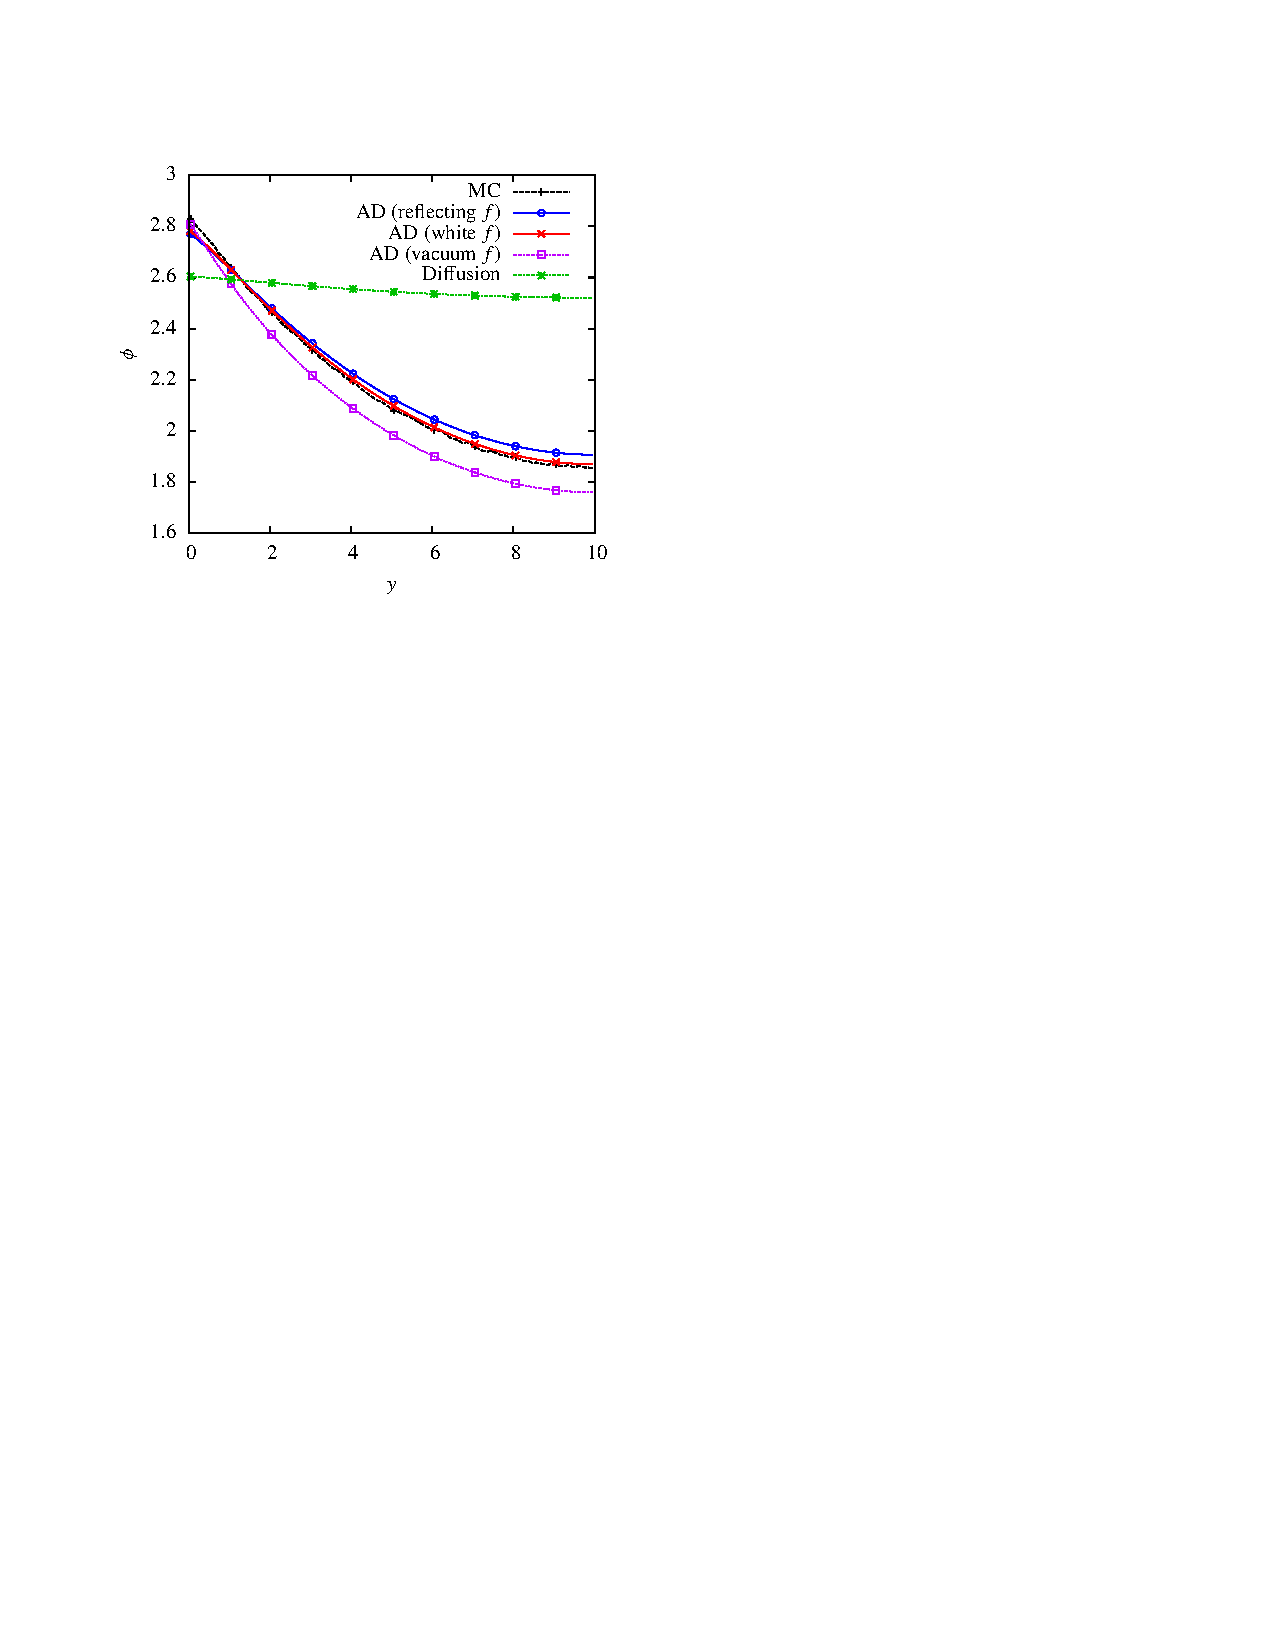
\includegraphics{example_figure}
  \caption{Captions are flush with the left.}
  \label{fig:voltage}
\end{figure}

Later on, we can include a table, even one that spans two columns such as
Table~\ref{tab:widetable}.
%%%%%%%%%%%%%%%%%%%%%%%%%%%%%%%%%%%%%%%%
\begin{table*}[htb]
  \centering
\begin{tabular}{llllllllll}\toprule
      & $\phi_T(0)$      & $\phi_T(10)$      & $\phi_T(20)$      &
      $\phi_D(0)$      & $\phi_D(10)$      & $\phi_D(20)$      & $\rho$      &
      $\varepsilon$      & $N_\text{it}$
\\ \midrule
$c=0.999$  & 0.9038 & 20.63 & 31.24 & 0.9087 & 20.63 & 31.23 & 0.2192 & $10^{-7}$ & 15
\\
$c=0.990$  & 0.3675 & 13.04 & 24.7 & 0.3696 & 13.04 & 24.69 & 0.2184 & $10^{-7}$ & 15
\\
$c=0.900$  & 0.009909 & 4.776 & 17.64 & 0.009984 & 4.786 & 17.63 & 0.2118 & $10^{-7}$ & 14
\\
$c=0.500$  & $6.069\times 10^{-5}$ & 2.212 & 15.53 & 6.213$\times 10^{-5}$ & 2.239 & 15.53 & 0.2068 & $10^{-7}$ & 13
\\
\bottomrule
\end{tabular}
  \caption{This is an example of a really wide table which might not normally
  fit in the document.}
  \label{tab:widetable}
\end{table*}
%%%%%%%%%%%%%%%%%%%%%%%%%%%%%%%%%%%%%%%%
Notice how the table reference uses a Roman numeral
for its numbering scheme, whereas the figure reference uses an Arabic numeral.
For one-column tables, use the \verb|table| environment; two-column tables use
\verb|table*|. The same applies to figures.

%%%%%%%%%%%%%%%%%%%%%%%%%%%%%%%%%%%%%%%%%%%%%%%%%%%%%%%%%%%%%%%%%%%%%%%%%%%%%%%%
\section{Conclusions}

Put your conclusions here. 

%%%%%%%%%%%%%%%%%%%%%%%%%%%%%%%%%%%%%%%%%%%%%%%%%%%%%%%%%%%%%%%%%%%%%%%%%%%%%%%%
\section{Acknowledgments}

This material is based upon work supported by ACDIS.

%%%%%%%%%%%%%%%%%%%%%%%%%%%%%%%%%%%%%%%%%%%%%%%%%%%%%%%%%%%%%%%%%%%%%%%%%%%%%%%%
\bibliographystyle{ans}
\bibliography{bibliography}
\end{document}
